
 \chapter{Parametric systems}\label{chapter addition of parameters}
% \chapter{Addition of parameters}

The infinite-state systems defined in the precedent chapter are widely used to model the behavior of computer programs. Essentially these approaches however address only concrete specifications.
For instance, one can ask, given a program, whether a certain set of states is reachable without some counter exceeding a threshold value $2048$, or one can ask whether a certain set of states is reachable after having more than $10$ time units elapse.
For certain types of computer programs however, such as embedded systems, the constraints depend on some environment, and concrete constraints are useful only when restricting oneself to a given concrete environment. 
In real life, it thus makes sense to rather ask, for instance, whether there exists a threshold value $t$ such that a certain set of states is reachable without some counter exceeding $t$, or to ask whether for all threshold $t$ a certain set of states is reachable after having more than $t$ time units elapse.
Hence the need to study under-specified systems, 
and parametric constraints. 
% For instance, one can wish to develop a model which allow to check that \textcolor{red}{an example: “message delivery within the time it takes to execute two assignment statements”}.

\iffalse
when studying the litterature on real time protocols, one sees that the desired timing properties for protocols are almost invariably parametric (cf [30,10,33]) because concrete timing constraints only make sense in the context of a given concrete environment

[10] H. Attiya, C. Dwork, N. Lynch and L. Stockmeyer. Bounds on the time to reach agreement in the presence of timing uncertainty. In Proc. 23 ACM STOC, 1991

[30] R. Strong, D. DOlev and F. Cristian. New latency bounds for atomic broadcast. In Proc. 11th IEEE RTSS, 1990.

[33] H. Weingberg and L. Zuck. Timed Ethernet: real-time formal specification of Ethernet. In Proc. 3r CONCUR, LNCS 630. Springer, 1992.
\fi
% Unfortunately, classical timed automata, where clocks can only be compared to constants, do not allow such a parametric reasoning.


In order to 
understand the behavior of such under-specified systems, Alur, Henzinger and Vardi have introduced parametric timed automata in their seminal paper \cite{AHV93-stoc}.
In addition to expressing concrete timing constraints, these can employ parametric constraints. Verification of the desired behavior of the system is then performed without concrete values. 
Their model laid the foundations for parametric reasoning about real time. 
% Parametric counter automata, defined in \cite{AHV93-stoc, annichini2000symbolic}, are similar to parametric timed automata. 
With similar considerations, it has also been natural to consider extensions of one-counter automata allowing updates that increase or decrease the counter by integer parameters \cite{IJTW93-icalp, BIL06-icalp}.


\iffalse
\cite{BIL06-icalp} Flat Parametric Counter Automata
\cite{IJTW93-icalp} New decidability results concerning two-way counter machines and applications. 
\fi
\iffalse
Work closely related to reachability in parametric one-counter automata is that of
Ibarra et al. [65], which shows decidability of reachability for a subset of the class of
deterministic parametric one-counter automata with sign tests. The decidability of
reachability over the whole class of such automata is stated as an open problem in
[65]. Note that although in this thesis parametric one-counter automata do not allow
negative counter values and sign tests, they allow non-determinism. Thus, the results
of this thesis are incomparable to those from [65]. 

[65] Oscar H. Ibarra, Tao Jiang, Nicholas Q. Trân, and Hui Wang. New decidability
results concerning two-way counter machines. SIAM Journal on Computing,
24(1):123–137, 1995.
\fi

In this thesis, we consider the problem of analysing parametric pushdown, one-counter and timed automata, i.e. automata extended with a stack, counter or clocks that can be compared with parameters.
These parameters can take unspecified values over infinite domains, which here consist in the set of words (for parametric pushdown automata) or the non-negative integers (for parametric one-counter automata and parametric timed automata). 
%
%
%
%
An {\em $\M$-parameter valuation} is then a function $\mu$ from a set $P$ of parameters to a 
% set $\Gamma^*$ of words
given set $\M$. We will omit the name of the set $\M$ in case it is obvious from context.
%
%
%
% or to the set $\N$ of non-negative integers, which can be seen as words over a unary alphabet.
Our interests lies in the parametric variants of 
%the problems of specification reachability games, parity games and emptyness. 
requirements such as safety or liveness properties: for instance, 
%to verify that the  model satisfies some safety or liveness property for at least one possible values of the parameters,
finding constraints on the parameters defining the set of all possible values for which the system satisfies a safety or liveness property, or verifying that the  
model satisfies some safety or liveness property for all possible values of the parameters.
% The latter problem can be solved, in the case of safety properties, as a parametric reachability problem. 

\section{Parametric reachability}

The {\em parametric reachability problem} for an automaton with parameters (e.g. for a PTA) asks whether there exists a parameter valuation
$\mu$ such that 
a final configuration of the resulting concrete automaton becomes
reachable.
From here onwards, we omit ``parametric'' and
write simply ``reachability problem'' when it is clear from context that the input automaton has parameters.
Solving such a problem can be useful to verify safety
properties of automaton with parameters, i.e. to answer the question ``is a bad state reachable for some valuation
of the parameters''?



We are interested in how adding a set of parameters influences decidability and complexity properties. 
In particular, notice that the effects of adding a set of parameters depend on the model. Indeed, the reachability problem for parametric timed automata is
long known to be undecidable~\cite{AHV93-stoc}, whereas the reachability problem for timed automata is
$\PSPACE$-complete \cite{alur1994theory}. On the other hand,
reachability for succinct one-counter automata %without non-zero tests 
is $\NP$-complete \cite{HKOW-09concur}
and
reachability for parametric %succinct 
one-counter automata %without non-zero tests
 is both $\NP$-hard and in $\NEXP$ \cite{haase2012complexity}.


\iffalse
In the 1990’s timed automata have been introduced by Alur and Dill [?]. They extend
finite automata by clocks that can be compared against integer constants and provide a popular
formalism to reason about the behavior of real-time systems with desirable algorithmic properties;
For a more general means to specify the behavior of under-specified systems, such as embedded
systems, Alur, Henzinger and Vardi [?] have introduced parametric timed automata (PTA).

for many applications of counter machines, including
modelling computer programs, it is natural to consider more general types of up-
dates, such as adding integer constants to a counter [3, 5, 16] or adding integer
parameters [4, 12]. Parametric automata are used in various synthesis problems,
and to model open programs, whose behaviour depends on values input from
the environment [2]. In [20] parameters are also used to model resources (e.g.,
time, memory, dollars) consumed by transitions. The reachability problem for
parametric counter automata asks whether there exist values of the parameters
such that a given configuration is reachable from another given configuration.
\fi



%\subsubsection{Parameter valuation game}
\section{Parametric games}

As noted precedently, 
several model checking problems can be
expressed as decision problems for games.
For instance 
\textcolor{black}{
as mentioned 
in the case of pushdown automata, 
}
the modal $\mu$-calculus
model checking problem is polynomially equivalent to solving the parity game problem.
% \textcolor{red}{Since the model checking problem has a more varied range of applications than the reachability problem (mb have a source for that or smtg)},
S%ince model checking is typically more involved than simply solving the reachability problem, and s
ince we are interested in parametric model checking and specification,
we are naturally interested in parametric variants of reachability games and parity games.

% finding constraints on the parameters defining the set of all possible values for which the system satisfies a safety or liveness property, or verifying that the model satisfies some safety or liveness property for all possible values of the parameters.

One goal may be to characterize the set of all possible parameter valuations for which a player has a winning strategy in a 
reachability game or a parity game
played on the arena induced by the
resulting concrete automaton
and some partition of its set of states. 
For determining such a set of parameter valuations, we incorporate the choice of the parameter valuation to the game. Each player then wants the parameter valuation to lead to an arena where it has a winning strategy.

In keeping with the spirit of alternation between players choosing successors in the arena, we consider here games where players
alternate choosing values for the parameters before alternating choosing successor configurations in the game on the induced arena.
For simplicity's sake, the values are assigned to the parameters one by one, alternating between values assigned by player $0$ and by player $1$.

A winning strategy for player $0$ allows to synthesize a controller that restricts the environment and ensures that {the property expressed by the winning condition always holds.}

\paragraph{Parameter valuation arenas}

We introduce here arenas over the set of partial $\M$-parameter valuations for a set of parameters
$P = P_0 \biguplus P_1$. The values are assigned to the parameters one by one, alternating between values assigned by player $0$ (corresponding to parameters in $P_0$) and by player $1$ (corresponding to parameters in $P_1$). Other options could have been considered: for instance, we could consider a fully existential approach 
(i.e. all parameters have their values assigned by player $0$), 
or a fully universal approach
(i.e. all parameters have their values assigned by player $1$). 
\iffalse
Note however that the alternating approach considered here encompasses both of the latter approaches: it suffices to include in the set $P$ parameters which do not appear in the rules of an automaton \---- or that appear only in rules that do not have any effect on whether or not a player has a winning strategy in reachability games or parity games played on resulting concrete automata \---- and to have a player assign values only to these ``unused'' parameters.  \\
\fi
Note however that the approach considered here encompasses both of the latter approaches:
the fully existential approach consists in the case where $P_1 = \emptyset$ and
the fully universal one, the case $P_0 = \emptyset$.


\iffalse
Given an ordering of the parameters $P = \{p_0, p_1, \ldots, p_k \}$ for some 
%\textcolor{red}{even}
 $k \in \N$, we partition the set of parameters into parameters with even numerotation, assigned to player $0$, and parameters with odd numerotation, assigned to player $1$.  
\fi

Assume an ordering of the parameters $P_0 \biguplus P_1 = \{p_0, p_1, \ldots, p_k \}$ for some 
%\textcolor{red}{even}
 $k \in \N$.
%
Then given a set $\M$, a {\em parameter valuation arena} is a tuple $A_{P_0,P_1,\M} = (S_0, S_1, \rightarrow_P)$ where
\begin{itemize}

\item $S_0$ is the set of all partial $\M$-parameter valuations with domain $\{p_0, p_1, \ldots, p_{j}\} \setminus \{p_j\}$ where $\p_j \in P_0$,

\item $S_1$ is the set of all partial $\M$-parameter valuations with domain $\{p_0, p_1, \ldots, p_{j}\} \setminus \{p_j\}$ where $\p_j \in P_1$,


\iffalse
\item $S_0$ is the set of all partial $\M$-parameter valuations with domain $\{p_0, p_1, \ldots, p_{2i+1}\}$ 
for some $i \in [0, \lceil k/2 \rceil - 1]$, plus the partial parameter valuation with domain $\emptyset$,
\item $S_1$ is the set of all partial $\M$-parameter valuations with domain $\{p_0, p_1, \ldots, p_{2i}\}$
for some $i \in [0, \lfloor k/2 \rfloor]$, and
\fi

\item
$ \mu \rightarrow_P \mu'$,
if $\mu' \in (\M)^{\{p_0, \ldots, p_j\}}$ for some $j \in [0,k]$,
$\text{Dom}(\mu) = \text{Dom}(\mu') \setminus \{p_j\}$
and
 $\mu'(p) = \mu(p)$ for $p \in \text{Dom}(\mu)$. \label{parametric arena}
\end{itemize}


Note that the arena has dead ends, and that these are the configurations that correspond to parameter valuations.
Given a strategy $\sigma_0$ for player $0$ and a strategy $\sigma_1 $ for player $1$,
the last configuration of the resulting play $\pi(\mu_\bot,\sigma_0, \sigma_1)$
is called {\em the resulting parameter valuation}
 and is denoted by $\mu_{\sigma_0, \sigma_1}$, where 
 $\mu_\bot$ is the partial parameter valuation with domain $\emptyset$. 
 %We do not really consider winning conditions for parameter valuation games. Rather, once the resulting parameter valuation is produced, it serves to instantiate the parametric transition system for the next game.


Parametric valuation arenas are used as prefixes in parametric games. Once the resulting parameter valuation is produced by the two players, it serves to instantiate the transition system for continuing the game.
%
%
Indeed, where a concrete automaton induces a transition system, a parametric automaton induces one transition system for every possible parameter valuation.
We use $T^\mu_\A$ to denote the transition system induced by the concrete automaton corresponding to
a parametric automaton $\A$ with parameters $P$ taking values in $\M$ and a parameter valuation $\mu: P \to \M$.


\iffalse
Then for a parametric automaton, and given a partition of its states,

Thus, for an  $n$-parametric pushdown automaton 
$\mathcal{Z}= (Q, \Gamma, P, R, q_{init}, \gamma_{init},F)$,
given a partition of
$Q$ into $Q_0$ and $Q_1$, 
we naturally partition the configurations of
%the transition system of 
 $\mathcal{Z}$
% $T^\mu_{\mathcal{Z}}$
into
$\Conf_{\mathcal{Z},0}=Q_0\times \Gamma^*$
and
$\Conf_{\mathcal{Z},1}=Q_1\times \Gamma^*$. 


With these notations in mind one can define the arena
$$
A_{(\mathcal{Z}, Q_0, Q_1, \mu)}
=
(\Conf_{\mathcal{Z},0}, \Conf_{\mathcal{Z},1}, \rightarrow_{\mathcal{Z},\mu})$$
induced by a PPDA $\mathcal{Z}$, a partition of its set of states, and a
parameter valuation $\mu: P\rightarrow \Gamma^*$. 

\fi

\begin{center}
	\begin{figure}
		\hspace{2cm}
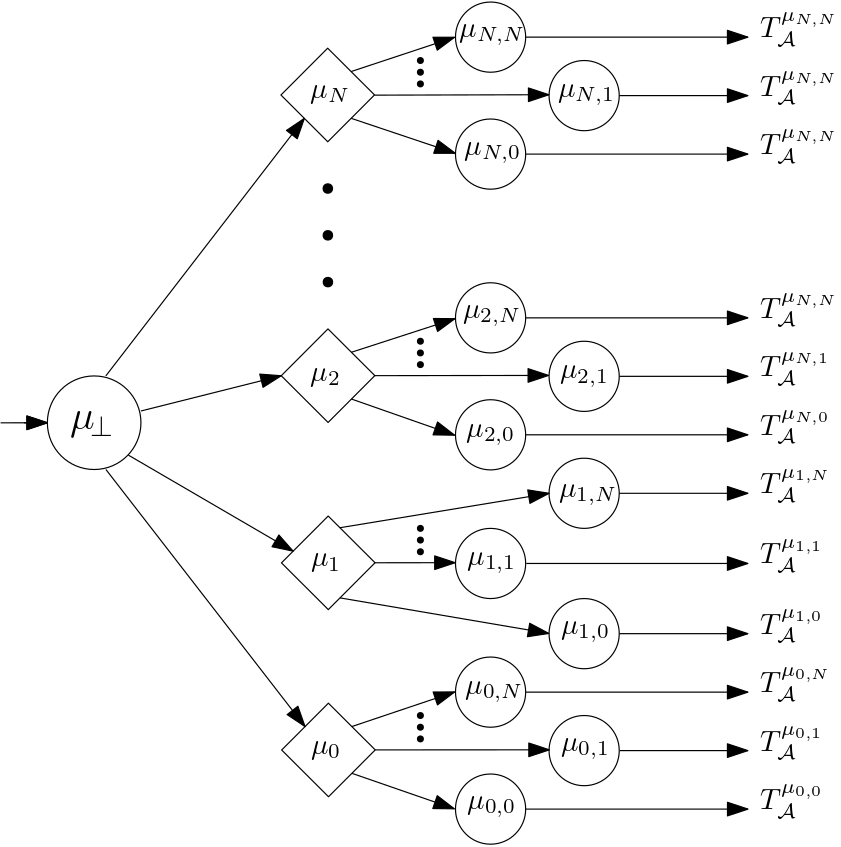
\includegraphics[width=0.7\textwidth]{figures/parameter_arena}
	\caption{An illustration of the arena for a parametric automaton $\A$ with 
%	two parameters, $p_0$ and $p_1$,	
	$P_0 = \{p_0\}$, $P_1 = \{p_1\}$ and
%	 that can take values in $[0,N]$ for some $N \in \N$. 
	$\M = [0,N]$ for some $N\in \N$.
	 Here $\mu_\bot$ is 
	%the partial parameter assignment with domain $\emptyset$,
	the totally undefined function and can be viewed rather as 
	the function that assigns $\bot$ to both parameters. For $i,j \in [0,N]$, $\mu_i$ is the partial parameter assignment with domain $\{p_0\}$ that maps $p_0$ to $i$ and $\mu_{i,j}$ is the parameter assignment that maps $p_0$ to $i$ and $p_1$ to $j$.
	 %Lastly $T^\mu_\A$ denotes the transition system induced by the concrete automaton corresponding to $\A$ with parameter valuation $\mu$.
	  As before, the circles belong to player $0$ and the diamonds to player $1$.} 
	\label{parametric_arena}
	\end{figure}
\end{center}




Given a parametric automaton $\A$ with a set of parameters $P = P_0 \biguplus P_1$ that can take 
values in the set $\M$,
a {\em parametric game} for $\A$ is a game played 
on the %following  arena $A_{\A}$.
%The 
arena $A_\A$
that include both 
% the configurations and transitions of
the parameter valuation arena
$A_{P_0, P_1,\M}$
and, % moreover contains 
for all parameter valuations $\mu: P\rightarrow \M$,
%the configurations and transitions of
the transition system %s 
% induced by the concrete automata corresponding to $\A$ with parameter valuation $\mu$
 $T_\A^\mu$
\---- albeit with configurations additionally indexed by $\mu$ %in the tuple
 to avoid confusion.
Moreover, for every 
dead end $\mu$
 in $A_{P_0,P_1,\M}$,
we add a transition
from the configuration $\mu \in \M^P$ to
$T_\A^\mu$.
See Figure~\ref{parametric_arena} for an illustration of such an arena.
Solving parametric games on an automaton with parameters (e.g. a POCA) then consists in answering whether there exists 
a winning strategy for player $0$
from the initial configuration of the parametric game.
Remark that the parametric reachability problem for an automaton with parameters can be seen as solving the parametric reachability game where $P_1 = \emptyset$, and $Q_1 = \emptyset$. 


\iffalse
Given a 
priority function $\Omega: Q \to [0, m]$,
we consider the function
$\widehat{\Omega}: \Conf(\mathcal{Z}) \cup (\Gamma^* \cup \bot)^{[0,n]} \to [0, m]$
where we set
$\widehat{\Omega}(q, w, \mu) = \Omega(q)$
for all				$w \in \Gamma^*$
and				for all $\mu \in (\Gamma^*)^{P}$,
and				$\widehat{\Omega}(\mu)=0$ for all $\mu \in (\Gamma^* \cup \bot)^{P}$.
\fi







